% Dans l'introduction, on présente le problème étudié et les buts
% poursuivis. L'introduction permet de faire connaître le cadre de la
% recherche et d'en préciser le domaine d'application. Elle fournit
% les précisions nécessaires en ce qui concerne le contexte de
% réalisation de la recherche, l'approche envisagée, l'évolution de
% la réalisation. En fait, l'introduction présente au lecteur ce
% qu'il doit savoir pour comprendre la recherche et en connaître la
% portée.
\Chapter{INTRODUCTION}\label{sec:Introduction}  % 10-12 lignes pour introduire le sujet.

\section{Context}\label{sec:context}

In the context of climate change and increasingly stringent environmental regulations, the aeronautical industry is moving toward the development of more efficient and lower-emission aircraft. This transition introduces new aerodynamic, structural, and operational challenges, while maintaining flight safety as the primary requirement. It also increases the need for reliable certification procedures capable of assessing aircraft performance and safety over a wide range of operating conditions.

Among the phenomena considered during aircraft certification, in-flight icing remains a major concern. Ice accretion occurs when an aircraft flies through clouds containing supercooled water droplets. When these droplets impinge on exposed surfaces and the local thermal conditions allow freezing, ice can accumulate on the aircraft geometry. The resulting ice shapes may significantly modify the aerodynamic configuration of the aircraft, leading to increased drag, reduced lift, altered stall behavior, and degraded controllability \cite{leary2002we,lynch2001effects,cao2015aircraft}. Ice accretion may also affect engines, probes, and sensors, as illustrated in Figure~\ref{fig:icingComp}, potentially producing erroneous measurements and compromising flight safety. Statistical analyses have shown that, in the United States between 1990 and 2000, approximately 12% of aircraft accidents caused by severe weather conditions were related to ice accretion \cite{baars2010review}.

\begin{figure}[htp]
\centering
\subfloat[Aircraft engine \cite{potapczuk2013aircraft}]{%
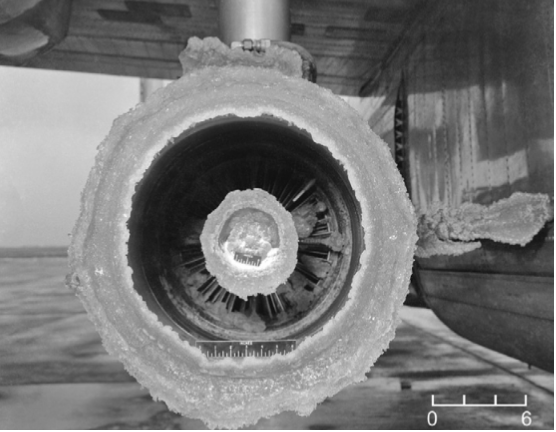
\includegraphics[width=0.325\textwidth]{FIGURES/Icing/engineIcing.png}%
\label{fig:icingEngine}%
}%
\hspace{1cm}%
\subfloat[Pitot probe \cite{noauthor_flight_nodate}]{%
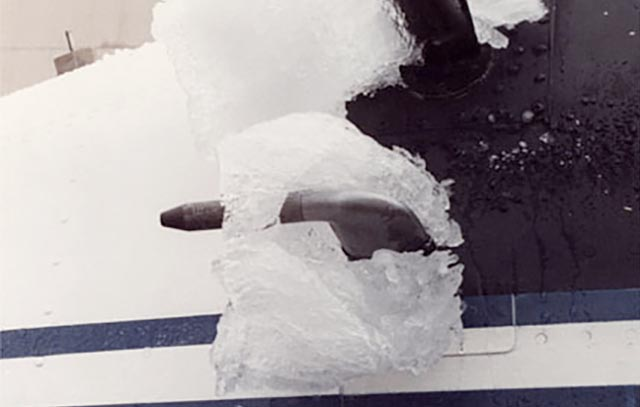
\includegraphics[width=0.4\textwidth]{FIGURES/Icing/pitotIcing.jpg}%
\label{fig:pitotIcing}%
}%
\caption{Examples of ice accretion on aircraft components.}
\label{fig:icingComp}
\end{figure}

The experimental investigation of aircraft icing has historically played a central role in understanding the physics of ice accretion and supporting certification activities. NASA, in particular, contributed significantly to this effort through the development of the Icing Research Tunnel (IRT), which enabled controlled experimental studies of ice formation on aerodynamic surfaces \cite{potapczuk1991icing}. These experiments provided essential data for the development, validation, and certification of aircraft icing prediction methods.

However, experimental icing certification presents significant practical challenges. These challenges become particularly important for modern large-scale aircraft configurations, where the physical size of the geometry may exceed the capabilities of existing icing wind tunnels. For example, the Common Research Model (CRM), considered during the second Ice Prediction Workshop (IPW2), required the use of hybrid or truncated wind-tunnel models, as shown in Figure~\ref{fig:CRM}. In such configurations, the full-scale leading-edge geometry is preserved while the afterbody is shortened or modified to fit within the wind-tunnel facility \cite{broeren2016ice}. Although necessary, this approach introduces additional complexity in model design, experimental setup, and interpretation of the results.

\begin{figure}[htp]
\centering
\subfloat[]{%
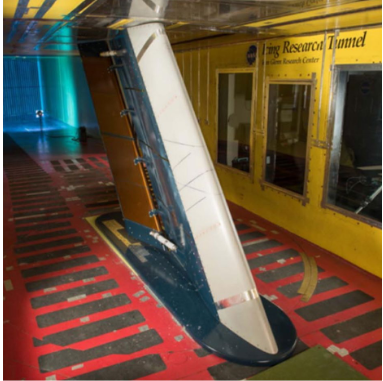
\includegraphics[width=0.325\textwidth]{FIGURES/CRM_WIND_TUNNEL.png}%
\label{fig:CRMWIND}%
}%
\hspace{1cm}%
\subfloat[]{%
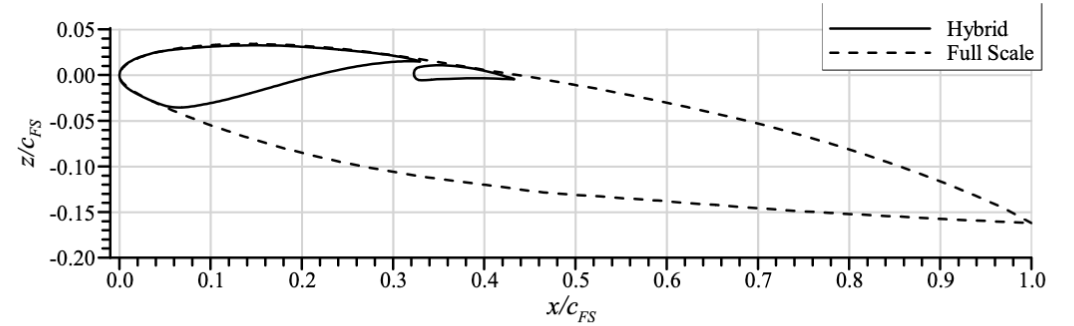
\includegraphics[width=0.6\textwidth]{FIGURES/CRM_HYBRID.png}%
\label{fig:CRNHYBRID}%
}%
\caption{CRM hybrid configuration used for wind-tunnel icing experiments \cite{broeren2016ice}.}
\label{fig:CRM}
\end{figure}

These limitations have motivated a growing interest in numerical prediction methods and digital certification strategies. When supported by rigorous verification and validation, numerical simulations can complement experimental campaigns, reduce testing costs, and provide detailed access to quantities that are difficult to measure experimentally. In the context of icing, numerical tools are particularly valuable because they allow the coupled effects of airflow, droplet transport, heat transfer, phase change, and geometry evolution to be investigated in a controlled and repeatable manner.

The complexity of icing certification has also increased with the introduction of Supercooled Large Droplet (SLD) conditions. Following the ATR-72 accident in 1994, additional attention was given to icing environments involving droplets larger than those traditionally considered in certification envelopes. This led to the introduction of Appendix O to the Federal Aviation Regulations in November 2014 \cite{appendixO}. Previous certification conditions, such as those covered by Appendix C, were primarily associated with supercooled standard droplets with diameters up to approximately 50~$\mu$m \cite{appendixC}. In contrast, SLD conditions involve much larger droplets, with characteristic diameters extending to several hundred micrometers and, in some cases, up to the millimeter range \cite{appendixO}. These conditions are often associated with freezing drizzle or freezing rain and may produce complex ice shapes, including horns, runback ice, and scalloped formations, as illustrated in Figure~\ref{fig:iceShapes}. The prediction of such three-dimensional ice shapes remains a challenging task and requires robust numerical methods capable of handling complex droplet impingement, thermodynamic behavior, and evolving geometries.

\begin{figure}[htp]
\centering
\subfloat[Clear-ice horns]{%
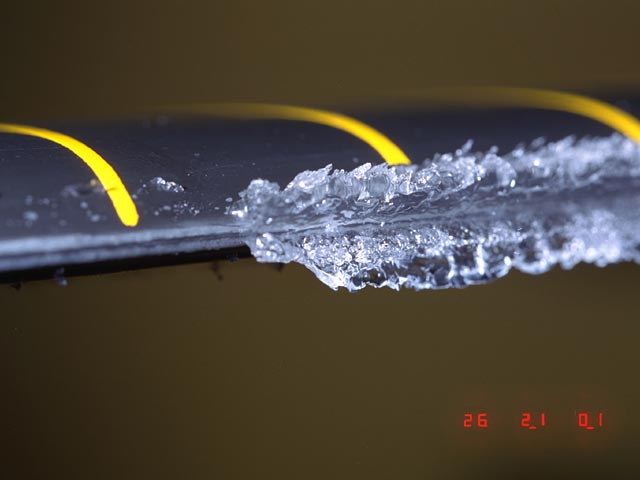
\includegraphics[width=0.35\textwidth]{FIGURES/Icing/iceHorns.jpg}%
\label{fig:iceHorns}%
}%
\hspace{1cm}%
\subfloat[Ice scallops]{%
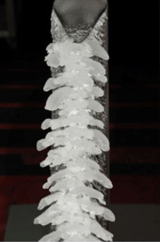
\includegraphics[width=0.175\textwidth]{FIGURES/Icing/iceScallops.png}%
\label{fig:iceScallops}%
}%
\caption{Examples of complex ice shapes obtained in the NASA IRT \cite{noauthor_glenn_nodate}.}
\label{fig:iceShapes}
\end{figure}

\section{Problem Statement}

Aircraft icing is a complex multiphysics phenomenon involving the interaction of aerodynamics, dispersed droplet transport, surface heat transfer, phase change, liquid water runback, and geometry deformation. From a numerical perspective, the main challenge is to predict the resulting ice shapes accurately and robustly, particularly for three-dimensional configurations and multilayer accretion processes. Recent Ice Prediction Workshops have shown that, despite significant progress, three-dimensional ice accretion prediction remains difficult and is not yet fully mastered \cite{laurendeau2022summary}.

The difficulty is not limited to the physical modeling itself. It also arises from the numerical treatment of the evolving geometry. As ice grows, the surface can develop sharp horns, thin features, highly curved regions, or complex three-dimensional patterns such as scallops. These features may degrade the quality of body-fitted meshes, introduce geometric intersections, or require repeated manual intervention during the remeshing process. Consequently, the robustness of the complete icing simulation workflow remains a critical limitation, especially when the objective is to perform automated multilayer simulations on realistic aircraft configurations.

\subsection{Ice Accretion Numerical Framework}

The ice accretion process is unsteady by nature. In practical icing solvers, it is commonly treated using a quasi-steady multilayer approach \cite{KIND1998257}. Under this assumption, the total icing time is divided into several time intervals, or layers. For each layer, the airflow, droplet impingement, surface thermodynamics, and geometry evolution are computed sequentially. The updated geometry is then used as the starting point for the next layer. This process is illustrated in Figure~\ref{fig:flowchart}.

The first step consists in computing the continuous air phase around the current geometry. This is commonly achieved by solving the Reynolds-Averaged Navier-Stokes equations. The airflow determines the aerodynamic loads, drives the droplet trajectories, influences the convective heat transfer, and affects the transport of liquid water along the surface \cite{BourgaultCote}.

The second step is the computation of the dispersed droplet phase. The droplet impingement distribution is a key input for the ice accretion model, since it determines where water is deposited on the surface. Droplet transport can be modeled using either Eulerian or Lagrangian approaches. In an Eulerian formulation, the droplet phase is treated as a continuous field governed by partial differential equations \cite{bourgault1999finite}. In a Lagrangian formulation, individual droplets or parcels are tracked through the flow field by solving their equations of motion \cite{rendall2014finite}. Each approach has advantages and limitations. Eulerian methods are generally efficient and well suited for dense impingement maps, whereas Lagrangian methods naturally provide trajectory-based information and can reduce numerical diffusion near impingement limits.

Once the droplet impingement distribution and convective heat-transfer information are available, the surface thermodynamic problem is solved. This step requires local mass and energy balances that account for water collection, evaporation, heat exchange, runback, and phase change. The solution provides the local ice growth rate or accumulated ice thickness over the current layer.

The final step consists in updating the geometry according to the predicted ice growth. Several techniques can be used for this purpose. Algebraic and Lagrangian deformation methods explicitly displace surface nodes, while implicit approaches, such as level-set methods, represent the evolving interface as the zero level of a signed-distance function \cite{bourgault-coteMultilayerAirfoilIce2019}. After the geometry has been updated, a new computational mesh may be generated for the next layer. This repeated update of the geometry and mesh is the basis of the multilayer ice accretion approach.

\begin{figure}[htp]
\centering
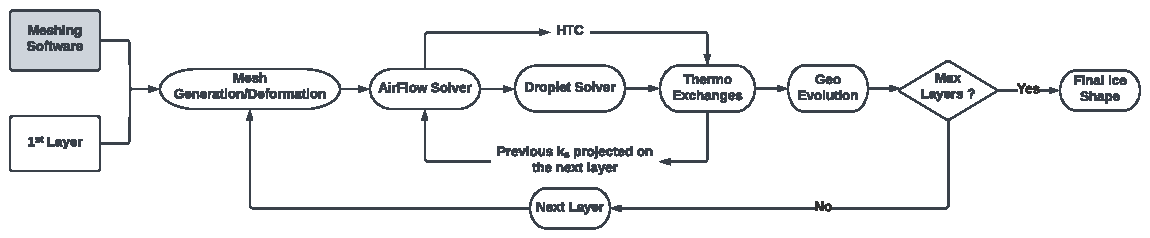
\includegraphics[width=1.0\textwidth]{FIGURES/flowchart.pdf}
\caption{Typical numerical framework for multilayer ice accretion simulations.}
\label{fig:flowchart}
\end{figure}

Although this framework is well established, the geometry evolution and remeshing stages remain particularly vulnerable. As illustrated in Figure~\ref{fig:overlap}, ice growth may generate surface overlaps, geometric intersections, or regions with insufficient mesh quality. Such failures can interrupt the multilayer loop and prevent the simulation from progressing. In two-dimensional configurations, local corrections and manual adjustments can sometimes be applied to recover a valid geometry. In three-dimensional simulations, however, these issues become significantly more complex due to the additional geometric degrees of freedom and the larger variety of possible ice shapes.

\begin{figure}[htp]
\centering
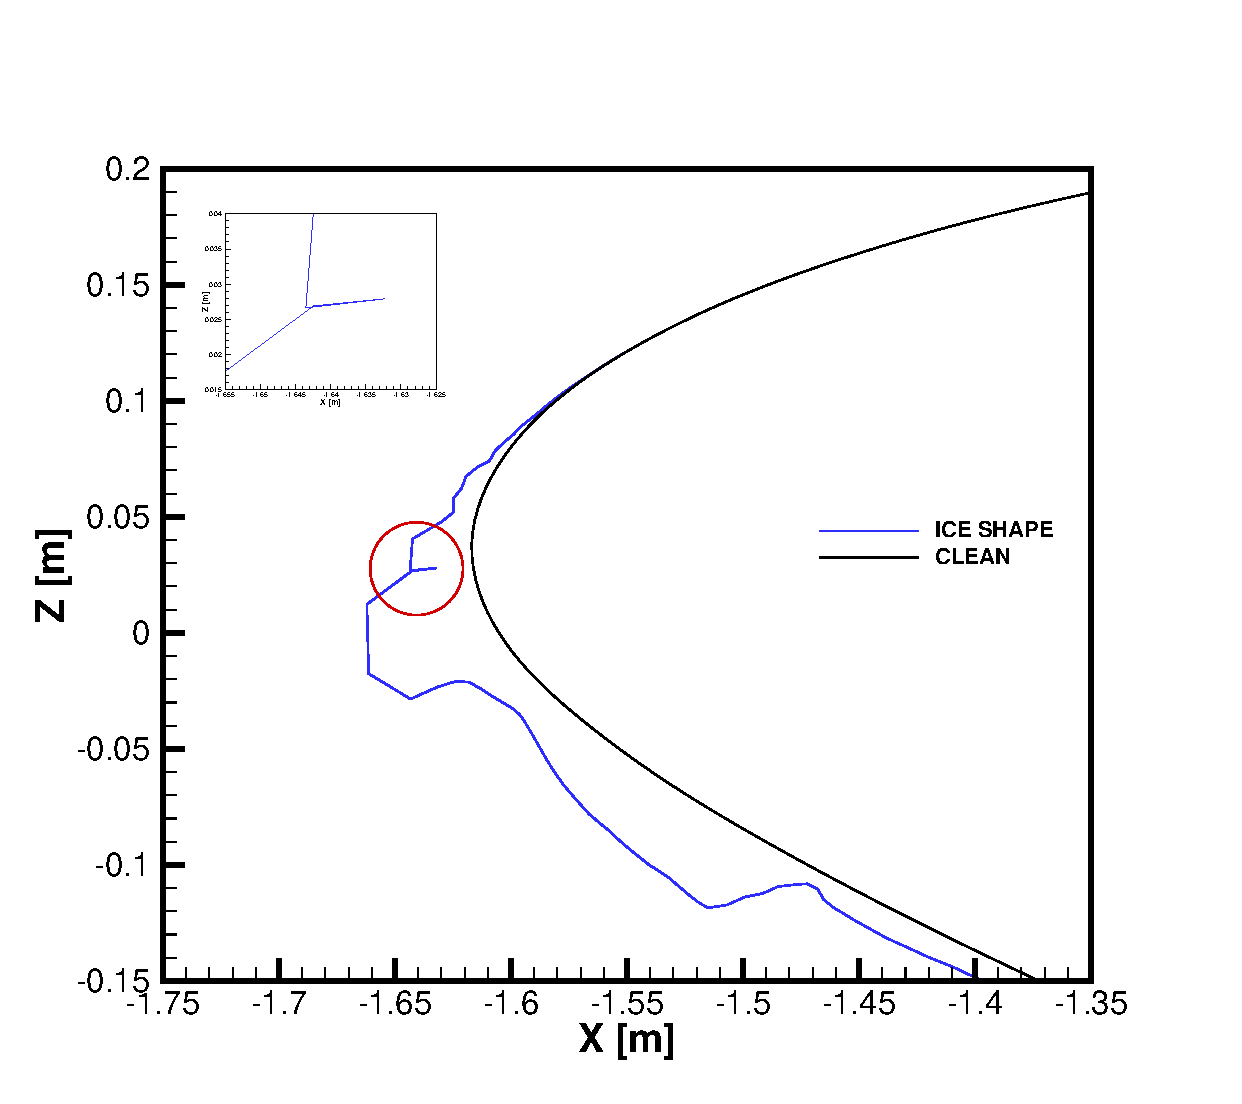
\includegraphics[width=.5\textwidth]{FIGURES/Icing/overlap.pdf}
\caption{Example of a simulation failure caused by a geometric intersection during ice growth.}
\label{fig:overlap}
\end{figure}

\subsection{Current Techniques and Potential Solution}

Most existing icing simulation frameworks rely on body-fitted meshes, in which the aircraft surface is explicitly represented as a boundary of the computational grid. This approach is natural and accurate when high-quality meshes can be generated. However, it becomes increasingly difficult for complex three-dimensional configurations, especially when the geometry evolves over several ice accretion layers.

Generating body-fitted meshes around clean aircraft geometries is already a challenging task. Structured grids are difficult to construct for complex topologies, while unstructured grids offer greater flexibility at the cost of larger memory requirements and increased computational expense. In addition, Reynolds-Averaged Navier-Stokes simulations require sufficient near-wall mesh quality to resolve or model the boundary layer accurately. This generally imposes constraints on the orthogonality, spacing, and smoothness of the first layers of cells near the wall \cite{BRUNO2022105351}. When ice accretes on the surface, the geometry becomes more irregular, and maintaining these mesh-quality requirements becomes even more difficult.

Immersed-boundary methods offer a possible way to reduce the dependence of the simulation on body-fitted mesh generation. In these methods, the solid geometry is represented independently of the background computational mesh, and boundary conditions are imposed through suitable numerical treatments. This approach can simplify the handling of complex and evolving geometries, since the geometry no longer needs to conform to the mesh. Combined with appropriate wall modeling, immersed-boundary methods can reduce the constraints associated with near-wall mesh generation and improve the robustness of the simulation workflow.

\begin{figure}[htp]
\centering
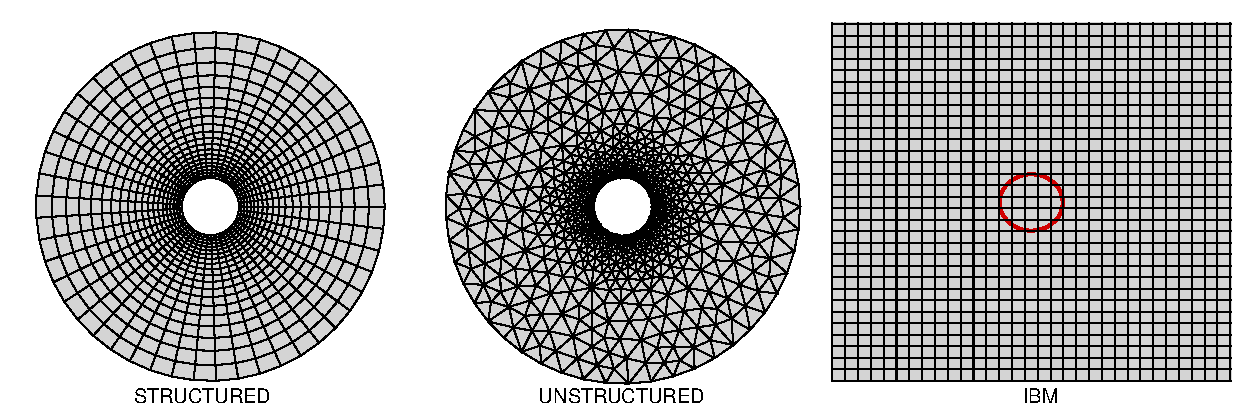
\includegraphics[width=1.0\textwidth]{FIGURES/Icing/IBM.pdf}
\caption{Comparison between a body-fitted mesh and a background mesh used in an immersed-boundary framework.}
\label{fig:IBM_MESH}
\end{figure}

Level-set methods provide another important tool for robust geometry evolution. By representing the ice surface implicitly, level-set methods can handle complex interface motion and provide a convenient framework for updating the ice shape. When combined with mesh adaptation or surface reconstruction techniques, they can support multilayer ice accretion simulations while reducing the risk of geometric inconsistencies.

The present work is therefore motivated by the need for robust numerical methods capable of predicting in-flight multilayer ice accretion on complex geometries. In particular, it focuses on the development and assessment of numerical approaches for droplet impingement, SLD effects, immersed-boundary modeling, and level-set-based geometry evolution within a multilayer ice accretion framework.

\section{Research Hypothesis}

The combination of advanced droplet-transport models, Supercooled Large Droplet effects, immersed-boundary techniques, wall modeling, and level-set-based geometry evolution can improve the robustness of multilayer ice accretion simulations while maintaining a level of accuracy comparable to established body-fitted approaches.

\section{Objectives}

\textbf{General Objective:}
Develop and assess robust numerical methods for in-flight multilayer ice accretion simulations.

\textbf{Specific Objectives:}

\begin{itemize}
\item Incorporate Supercooled Large Droplet effects into the ice accretion framework;
\item Develop and evaluate Eulerian and Lagrangian droplet-transport approaches for droplet impingement prediction;
\item Improve the robustness of ice-shape generation for complex and evolving geometries;
\item Assess the use of level-set methods for multilayer ice accretion and geometry evolution;
\item Examine the feasibility of immersed-boundary techniques for reducing the constraints associated with body-fitted remeshing;
\item Evaluate the accuracy, robustness, and efficiency of the proposed methods against reference numerical and experimental data.
\end{itemize}

\section{Requirements and Constraints}

The proposed methodology must satisfy the following requirements:

\begin{itemize}
\item The numerical methods must be applicable to complex two-dimensional and three-dimensional icing configurations;
\item The multilayer process must remain robust for evolving ice geometries;
\item The workflow should minimize user intervention during geometry update and mesh generation;
\item The proposed methods should not significantly compromise the accuracy of the predicted impingement distributions or ice shapes;
\item The methodology should remain compatible with practical computational resources used for aircraft icing simulations.
\end{itemize}

\section{Thesis Outline}

This thesis is organized as follows. Chapter~\ref{sec:LiteratureReview} presents a review of the main physical and numerical models used in aircraft ice accretion simulations, with particular attention to droplet impingement, SLD effects, immersed-boundary techniques, and level-set methods. Chapter~\ref{sec:Methodology} describes the numerical methodology developed in this work. The following chapters present verification and validation studies for the droplet-transport models, immersed-boundary formulation, and level-set-based geometry evolution. Finally, the thesis concludes with a summary of the main contributions, limitations, and perspectives for future work.
